\section{Baseline Comparison}

\autoref{fig:data-terrain-evaluation-comparison} shows the performance
of GaitNet compared to the baseline method across a variety of terrain
difficulties and commanded velocities. The results indicate that GaitNet
outperforms the baseline method in most scenarios, particularly in more
challenging terrains and at higher commanded speeds. This demonstrates
the effectiveness of GaitNet in generating robust gaits that can adapt
to varying conditions.

Further analyzing these graphs, we can see that GaitNet maintains excellent
performance when the commanded velocity is under 0.15\,m/s or the terrain
difficulty is below 5\%. ContactNet on the other hand, begins to degrade in
performance for commanded velocities above 0.05\,m/s and increasingly with
terrain difficulties. GaitNet's superior performance in these scenarios
highlights the advantages of its dynamic and acyclic gait generation
capabilities.

\begin{figure}[H]
  \centering
  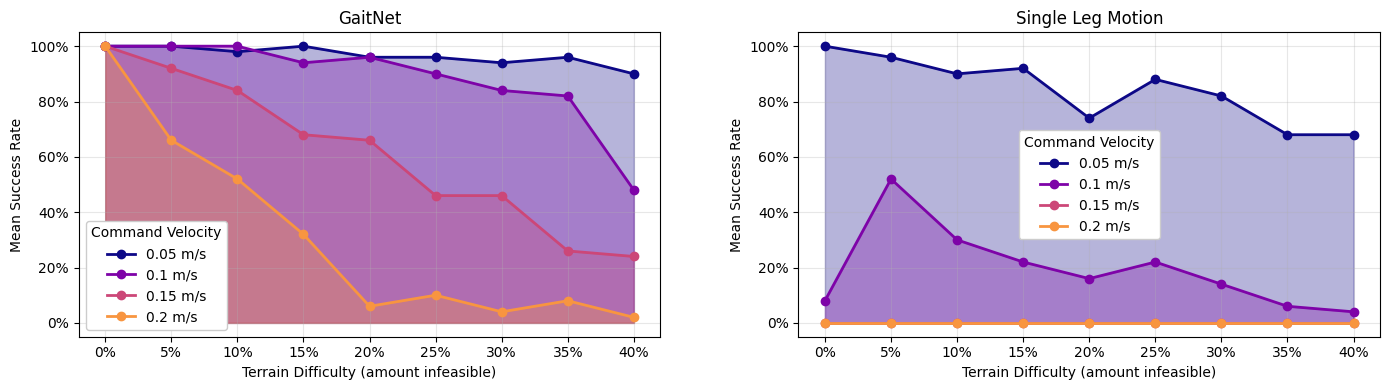
\includegraphics[width=\textwidth]{images/data/terrain-evaluation-comparison.png}
  \caption{Evaluation of GaitNet and the baseline method for
  different terrain difficulties and commanded velocities.}
  \label{fig:data-terrain-evaluation-comparison}
\end{figure}
